\documentclass{article}
\usepackage{amsmath} % import of math elements
\usepackage{mathtools} %import of other math elements
\usepackage{tikz} 
\usetikzlibrary{shapes,positioning,calc} 

%-------------------------------------------------------
% Document information
%-------------------------------------------------------

\title{Robbot project documentation} %Title 

\author{Roberto \textsc{Antoniello}} %author name

\begin{document}
\maketitle % show the title and author and date
%-------------------------------------------------------
%Introduction
%-------------------------------------------------------

\begin{center} In this file I resume how Robbot works with more details than the README file you can find in the repository.
Robbot is a Telegram bot with a bunch of different features. Some of them extend the use of Telegram you usually do, some of them are just funny features.\\
The bot is written in Python and it is running in Python3.8 at the moment.\end{center}

%-------------------------------------------------------
%First section about configuration file
%-------------------------------------------------------
\section{Configuration file}

The configuration file is the first thing you must check because without it well compiled, the bot won't run at all. This file is also well explained in README file so I won't spend a lot of words on it.
\begin{center} $config-example.json \Rightarrow config.json$ \end{center}

\subsection{DB path}
The .db file will be saved in the directory you choose and set in config.json file
\begin{center} $"path-db" \Rightarrow config.json$ \end{center}

\subsection{Super admin data}
In this section we put our Telegram data as super admin(the only one) of the bot. The super admin is able to manage the db changes such as adding users, promote to admin and deleting users/revoke admin powers.
\begin{center} $"id-super-admin" \Rightarrow config.json$ \end{center}

\subsection{commands,admin commands and super}
Here we put the name of commands the bot is able to recognize and execute. For example if we don't want to execute the weather we just don't put it on user-commands field. It's the same for admin and super commands.
\begin{center} $"user-commands" \Rightarrow config.json$ \\
               $"admin-commands" \Rightarrow config.json$ \\
               $"super-admin-commands" \Rightarrow config.json$
\end{center}

%-------------------------------------------------------
%Second section about app.py(main)
%-------------------------------------------------------
\section{Main}
app.py is the main source file. It creates the session, it connects with Telegram API using Pyrogram Client class and it's in constant wait for arriving messages.
First of all it fetches the information from configuration file, then it starts the connection.
While waiting, the bot will ignore any messages it doesn't recognize as a known command. Otherwise if it's a known command, it checks for permission to the user launched that command. If it's a recognized user, the entire message will be managed by a parser function and passed to a specific fetch function written inside controller.py.
If a command isn't launched by a registered user, the bot will reply with a default message.
\begin{center} $app.py \xrightarrow{\text{command}} controller.py$ \end{center}

%-------------------------------------------------------
%Third section about the controller
%-------------------------------------------------------
\section{Controller}
Just like in the MVC design pattern, this controller takes the input arriving from the main and it calls the right function in the right source file in $utils$ and $modules$ folders. How it works? \\
There are three dictionaries dedicated to the three types of command(user,admin,super). The key is the command and the value is the path of function it executes. As said in Main section, here we have the fetch command functions matched with the dictionaries mentioned in the previous row. The specific function will return a sendMessage and then the main will wait for the next command.
\begin{center} $controller.py \xrightarrow{\text{command fetched}} (modules \ or \ utils)$ \end{center}

\subsection{parser function}
This simple function mentioned in the first section takes the input message as argument and it deletes the command at the beginning, returning then just the query that will be sended by the controller to the right module which will manage and execute it.

\subsection{other details}
Inside the controller there is also a small function(visualizza) which print the current state of the incoming message on terminal such as a live log. \\

%-------------------------------------------------------
%4th section about the get_config source file
%-------------------------------------------------------
\section{get-config}
this source file contains some support functions that are often used in many situations. The first one return in a variable the content of the configuration file to get the fields easily. \\
The remaining functions are all about Telegram features such as getting information from the json message or renaming for example the send-message of Pyrogram to avoid including the decorator in every source file and just call this one by including get-config.
\begin{center} $app.py \xrightarrow{\text{get-config-file()}} running$ \end{center}

%-------------------------------------------------------
%5th section about the sysfunctions source file
%-------------------------------------------------------
\section{sysfunctions}
This file contains functions using directly Telegram features such as the poll function or get-message. It also includes the help function.

\section{Summary till now}
\begin{center} $app.py \xrightarrow{\text{get-config-file()}} running$ \end{center}
\begin{center} $app.py \xrightarrow{\text{command}} controller.py$ \end{center}
\begin{center} $controller.py \xrightarrow{\text{command fetched}} (modules \ or  \ utils)$ \end{center}
\begin{center} $(modules \ or \ utils) \xrightarrow{\text{return message}} app.py$ \end{center}
\begin{center} $app.py \xrightarrow{\text{waiting for the next command}} app.py$ \end{center}

%-------------------------------------------------------
%6th section about database
%-------------------------------------------------------
\section{Database}
In this section we'll focus about the database structure. There are two main table: User and Stats. \\ 
the first one saves data of users such as Telegram id(to check if it's registered) and a couple of boolean fields for admin rights.\\
The Stats table is linked to the User one by the id field and it saves information about how many times a command is used by every users.
There's also a Group table but it's not used at the moment, maybe in the future or not at all and it will be deleted in that case.\\

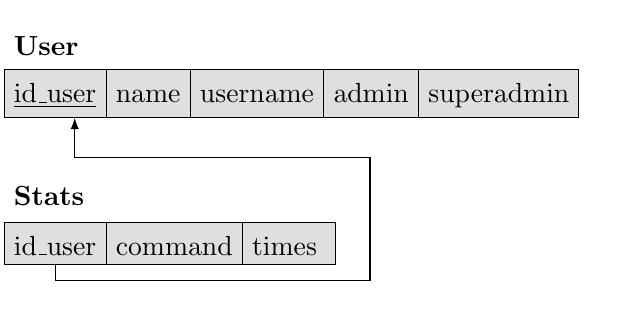
\begin{tikzpicture}[relation/.style={rectangle split, rectangle split parts=#1, rectangle split part align=base, draw, anchor= center, align=center, text height=3mm, text centered}]\hspace*{-0.3cm}

\node (usertitle) {\textbf{User}};
\node [relation=5, rectangle split horizontal, rectangle split part fill={lightgray!50}, anchor= north west, below=0.6cm of usertitle.west,anchor=west] (user)
	{\underline{id\_user} 
	\nodepart{two} name
	\nodepart{three} username
	\nodepart{four} admin
	\nodepart{five} superadmin};

\node [below=1.3cm of user.west,anchor=west] (statstitle) {\textbf{Stats}};
\node [relation=3,rectangle split horizontal, rectangle split part fill ={lightgray!50}, below=0.6cm of statstitle.west,anchor=west] (stats)
	{\nodepart{one} id\_user
	 \nodepart{two} command
	 \nodepart{three} times };

\draw[-latex] (stats.one south) -- ++(0,-0.2) -| ($(stats.one south) + (4,0)$) |- ($(user.one south) + (0.25,-0.50)$) -| ($(user.one south) + (0.25,0)$);

\end{tikzpicture}


\end{document}
